\begin{post}
	\postdata{NRB}{2011}{10}{07}{23}{45}{37}
	\begin{content}
NRB stands for Norebang ({\H 노래방}), which is a combination of song ({\H 노래}) and room ({\H 방}). So, who knows what a song room is? You? Or you? Nobody? OK, I'll tell you{\ldots}it's KARAOKE!

\begin{wrapfigure}{l}{0.38\textwidth}
\vspace{-12pt}\centering\fbox{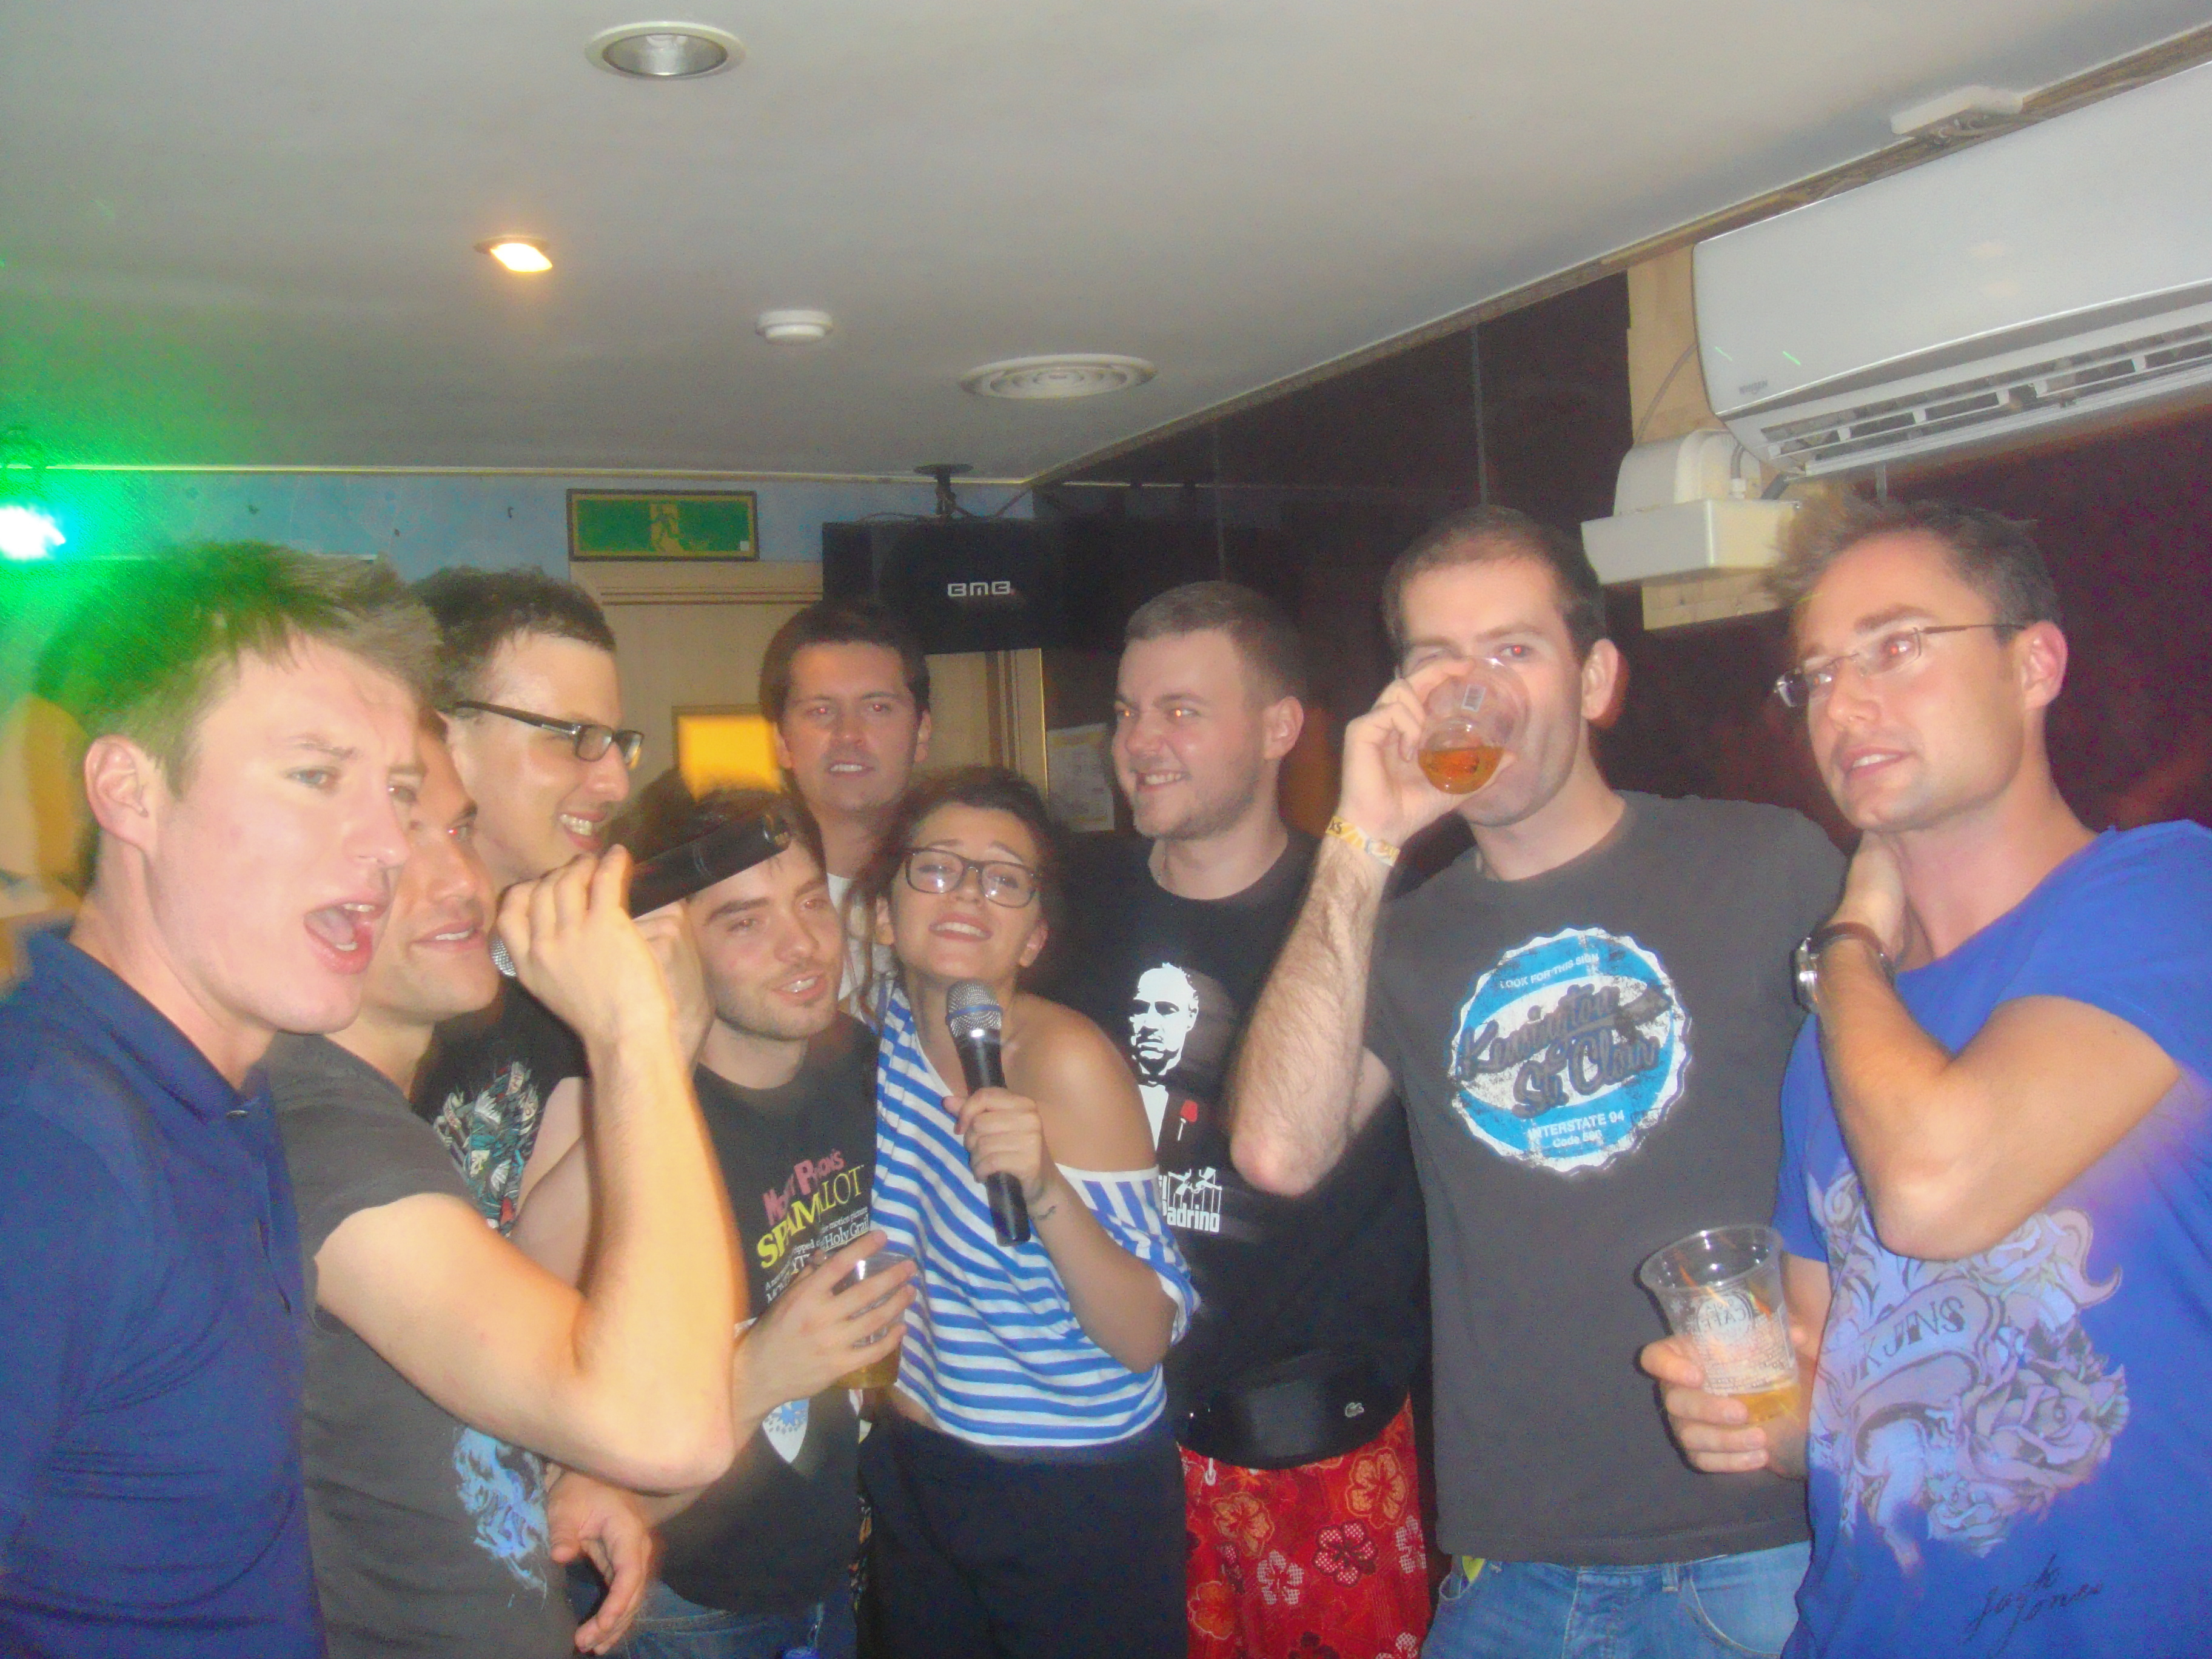
\includegraphics[height=140pt]{photos/10/07/DSC02450.jpg}}
\vspace{-24pt}
\end{wrapfigure}On one September night we have decided to go for some karaoke. South Korea is, as almost all Asian countries, crazy about karaoke and singing. There are about 35,000 Norebangs in Korea, and they are an integral part of South Korean culture. A typical evening might start with a Korean BBQ (bulgogi) with few bottles of soju or makkoli, then a ``Soju and hof'' bar (basically soju and beer) and when everybody is drunk and nearly unconscious, they go to a Norebang to sober up and have some fun. We chose the more direct way --- from our dorm directly to the norebang. Even though our campus is located in not that cool part of Seoul, there are about 6 karaoke places within the walking distance, which is awesome. We were quite a big group (approx. 15 people), so it was guaranteed that we will have a good time. And we indeed had.

The karaoke room was quite ``normal'' --- sofa, table, TV, speakers, remote control. And 3 books with songs in English, Korean, Japanese, Chinese, Spanish, Russian and quite a few other languages.

At the beginning, when everybody was sober, nobody wanted to sing. That is understandable, though, since we did not know each other that well and embarrassing yourself in front of other people requires either big balls or big bowls of alcohol. We chose the second way, so we started ordering beers and soju to get the party started. If I remember correctly, the first volunteer was Simone or Mario, however, soon after the first performance everybody got into the right mood and the hell has broken loose.

\begin{figure}[h]
\centering
\subfigure{\fbox{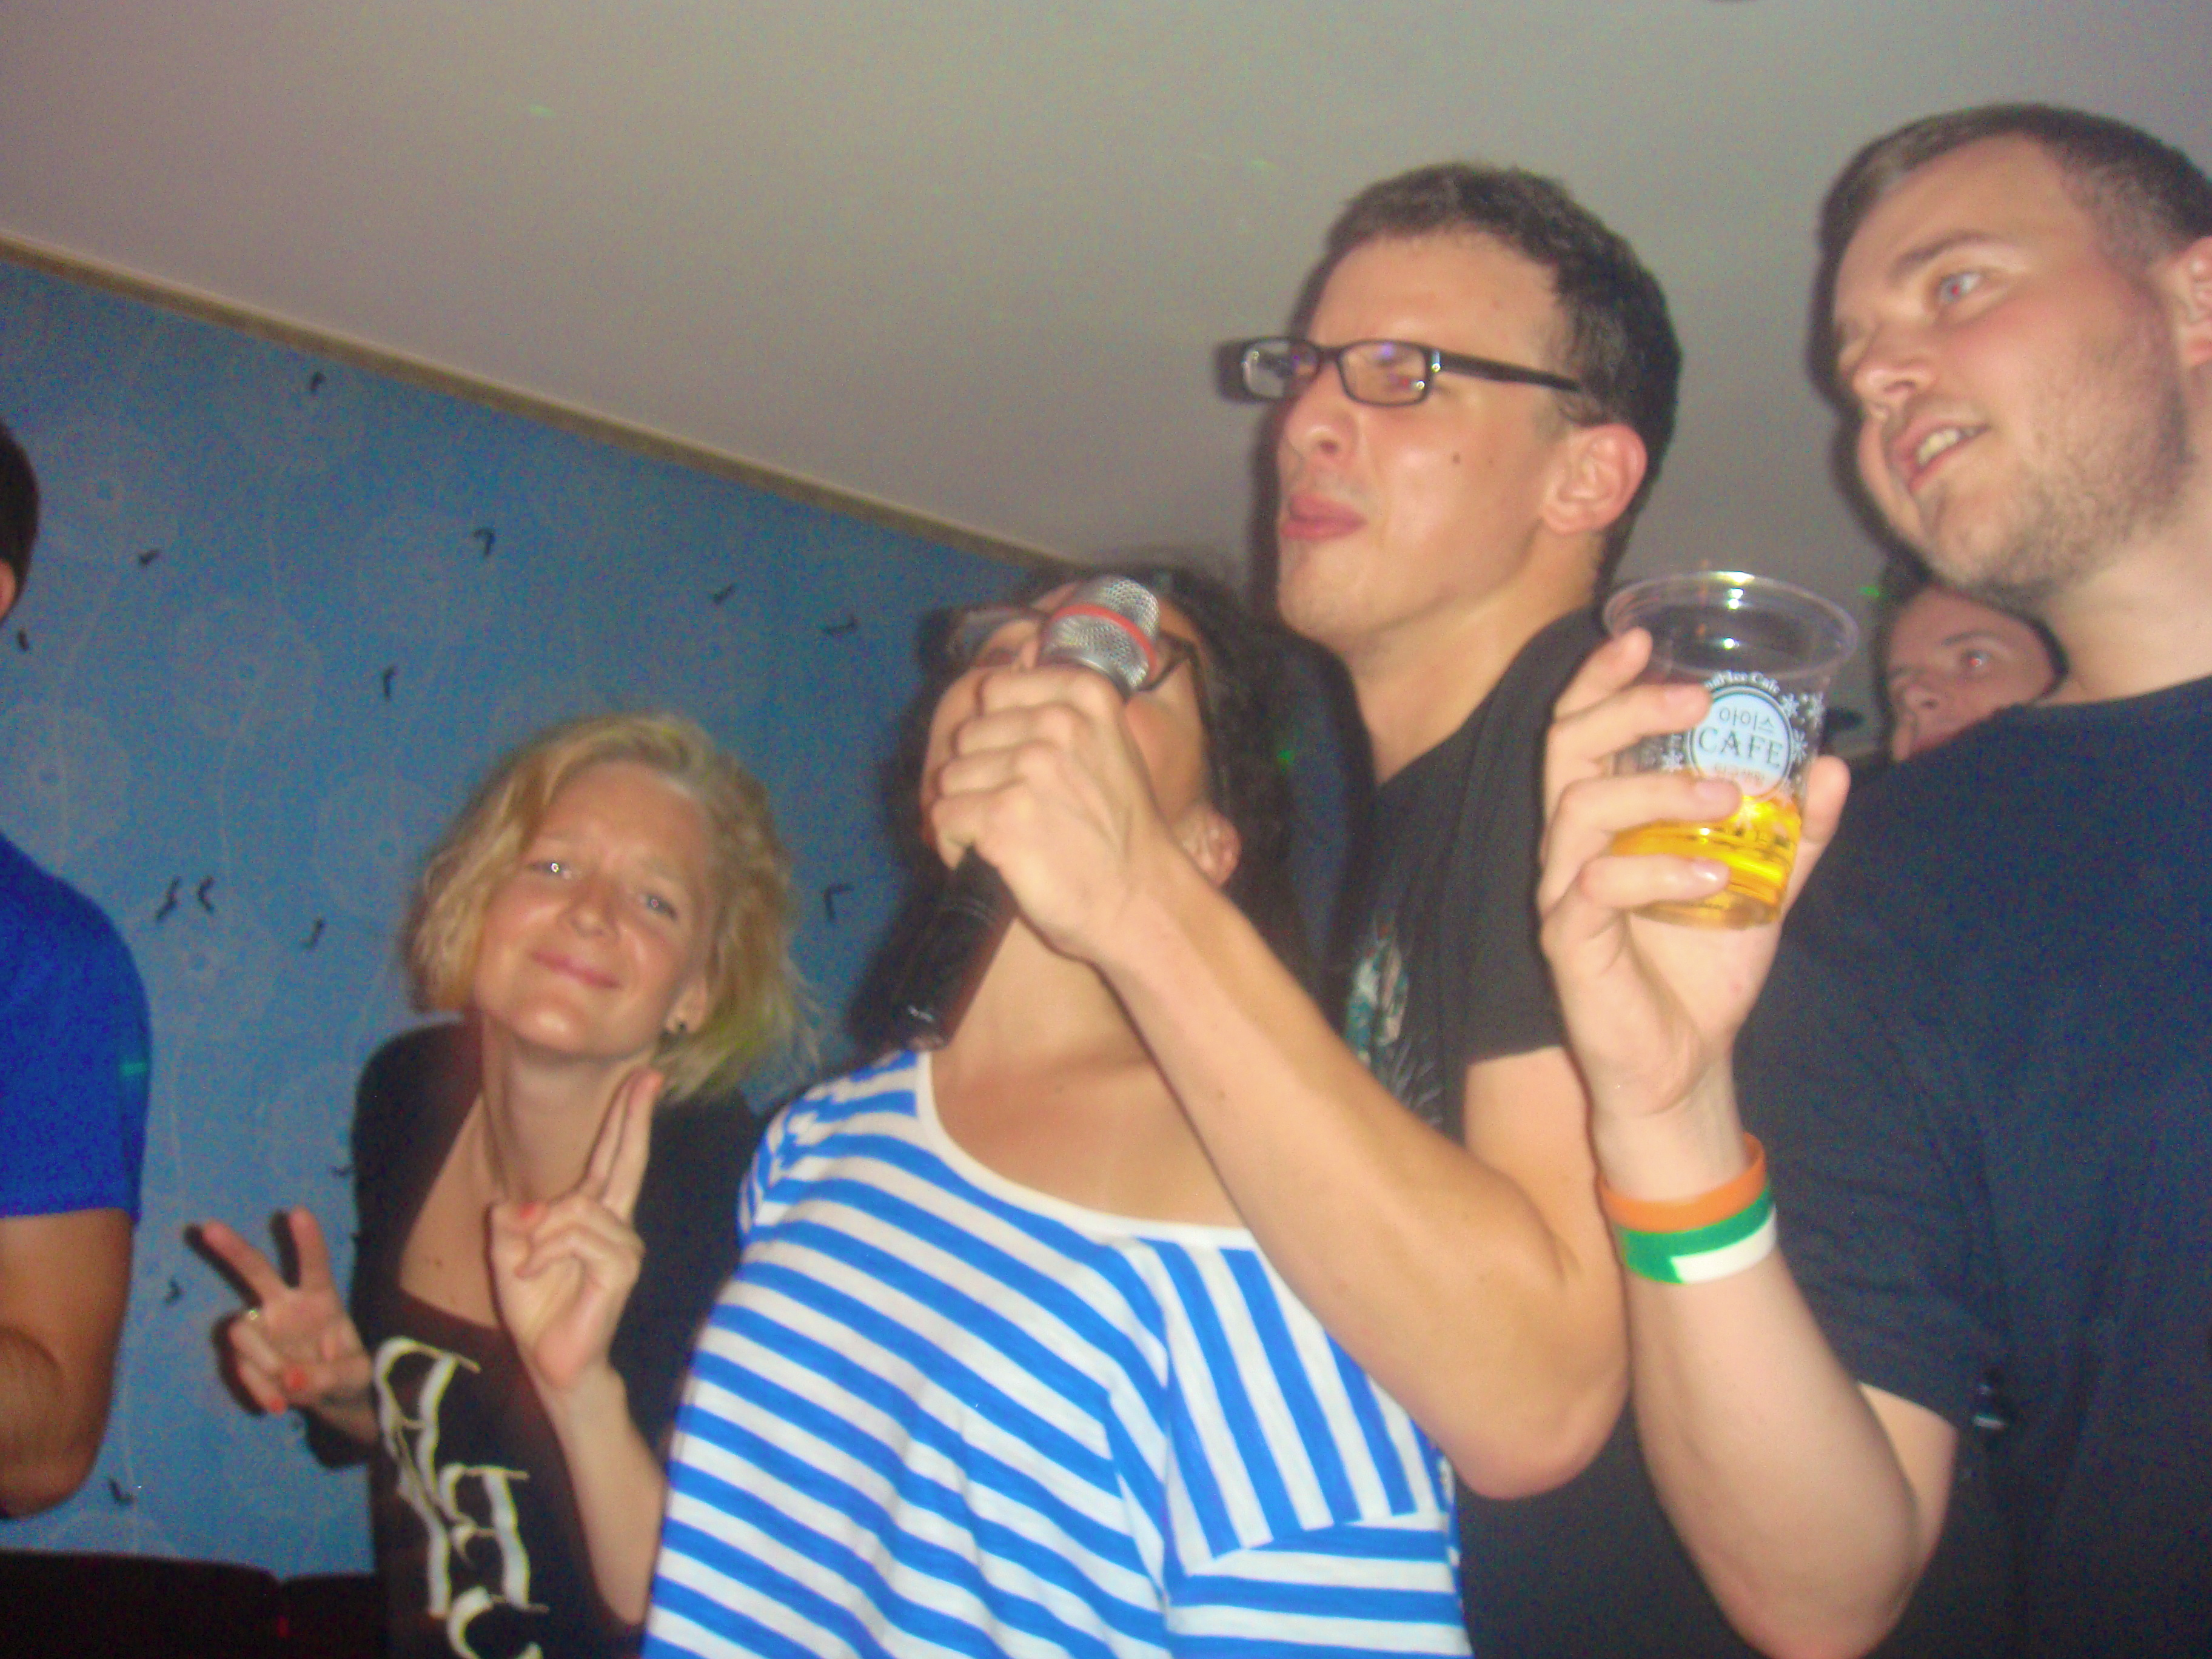
\includegraphics[width=0.43\textwidth]{photos/10/07/DSC02440.jpg}}}
\subfigure{\fbox{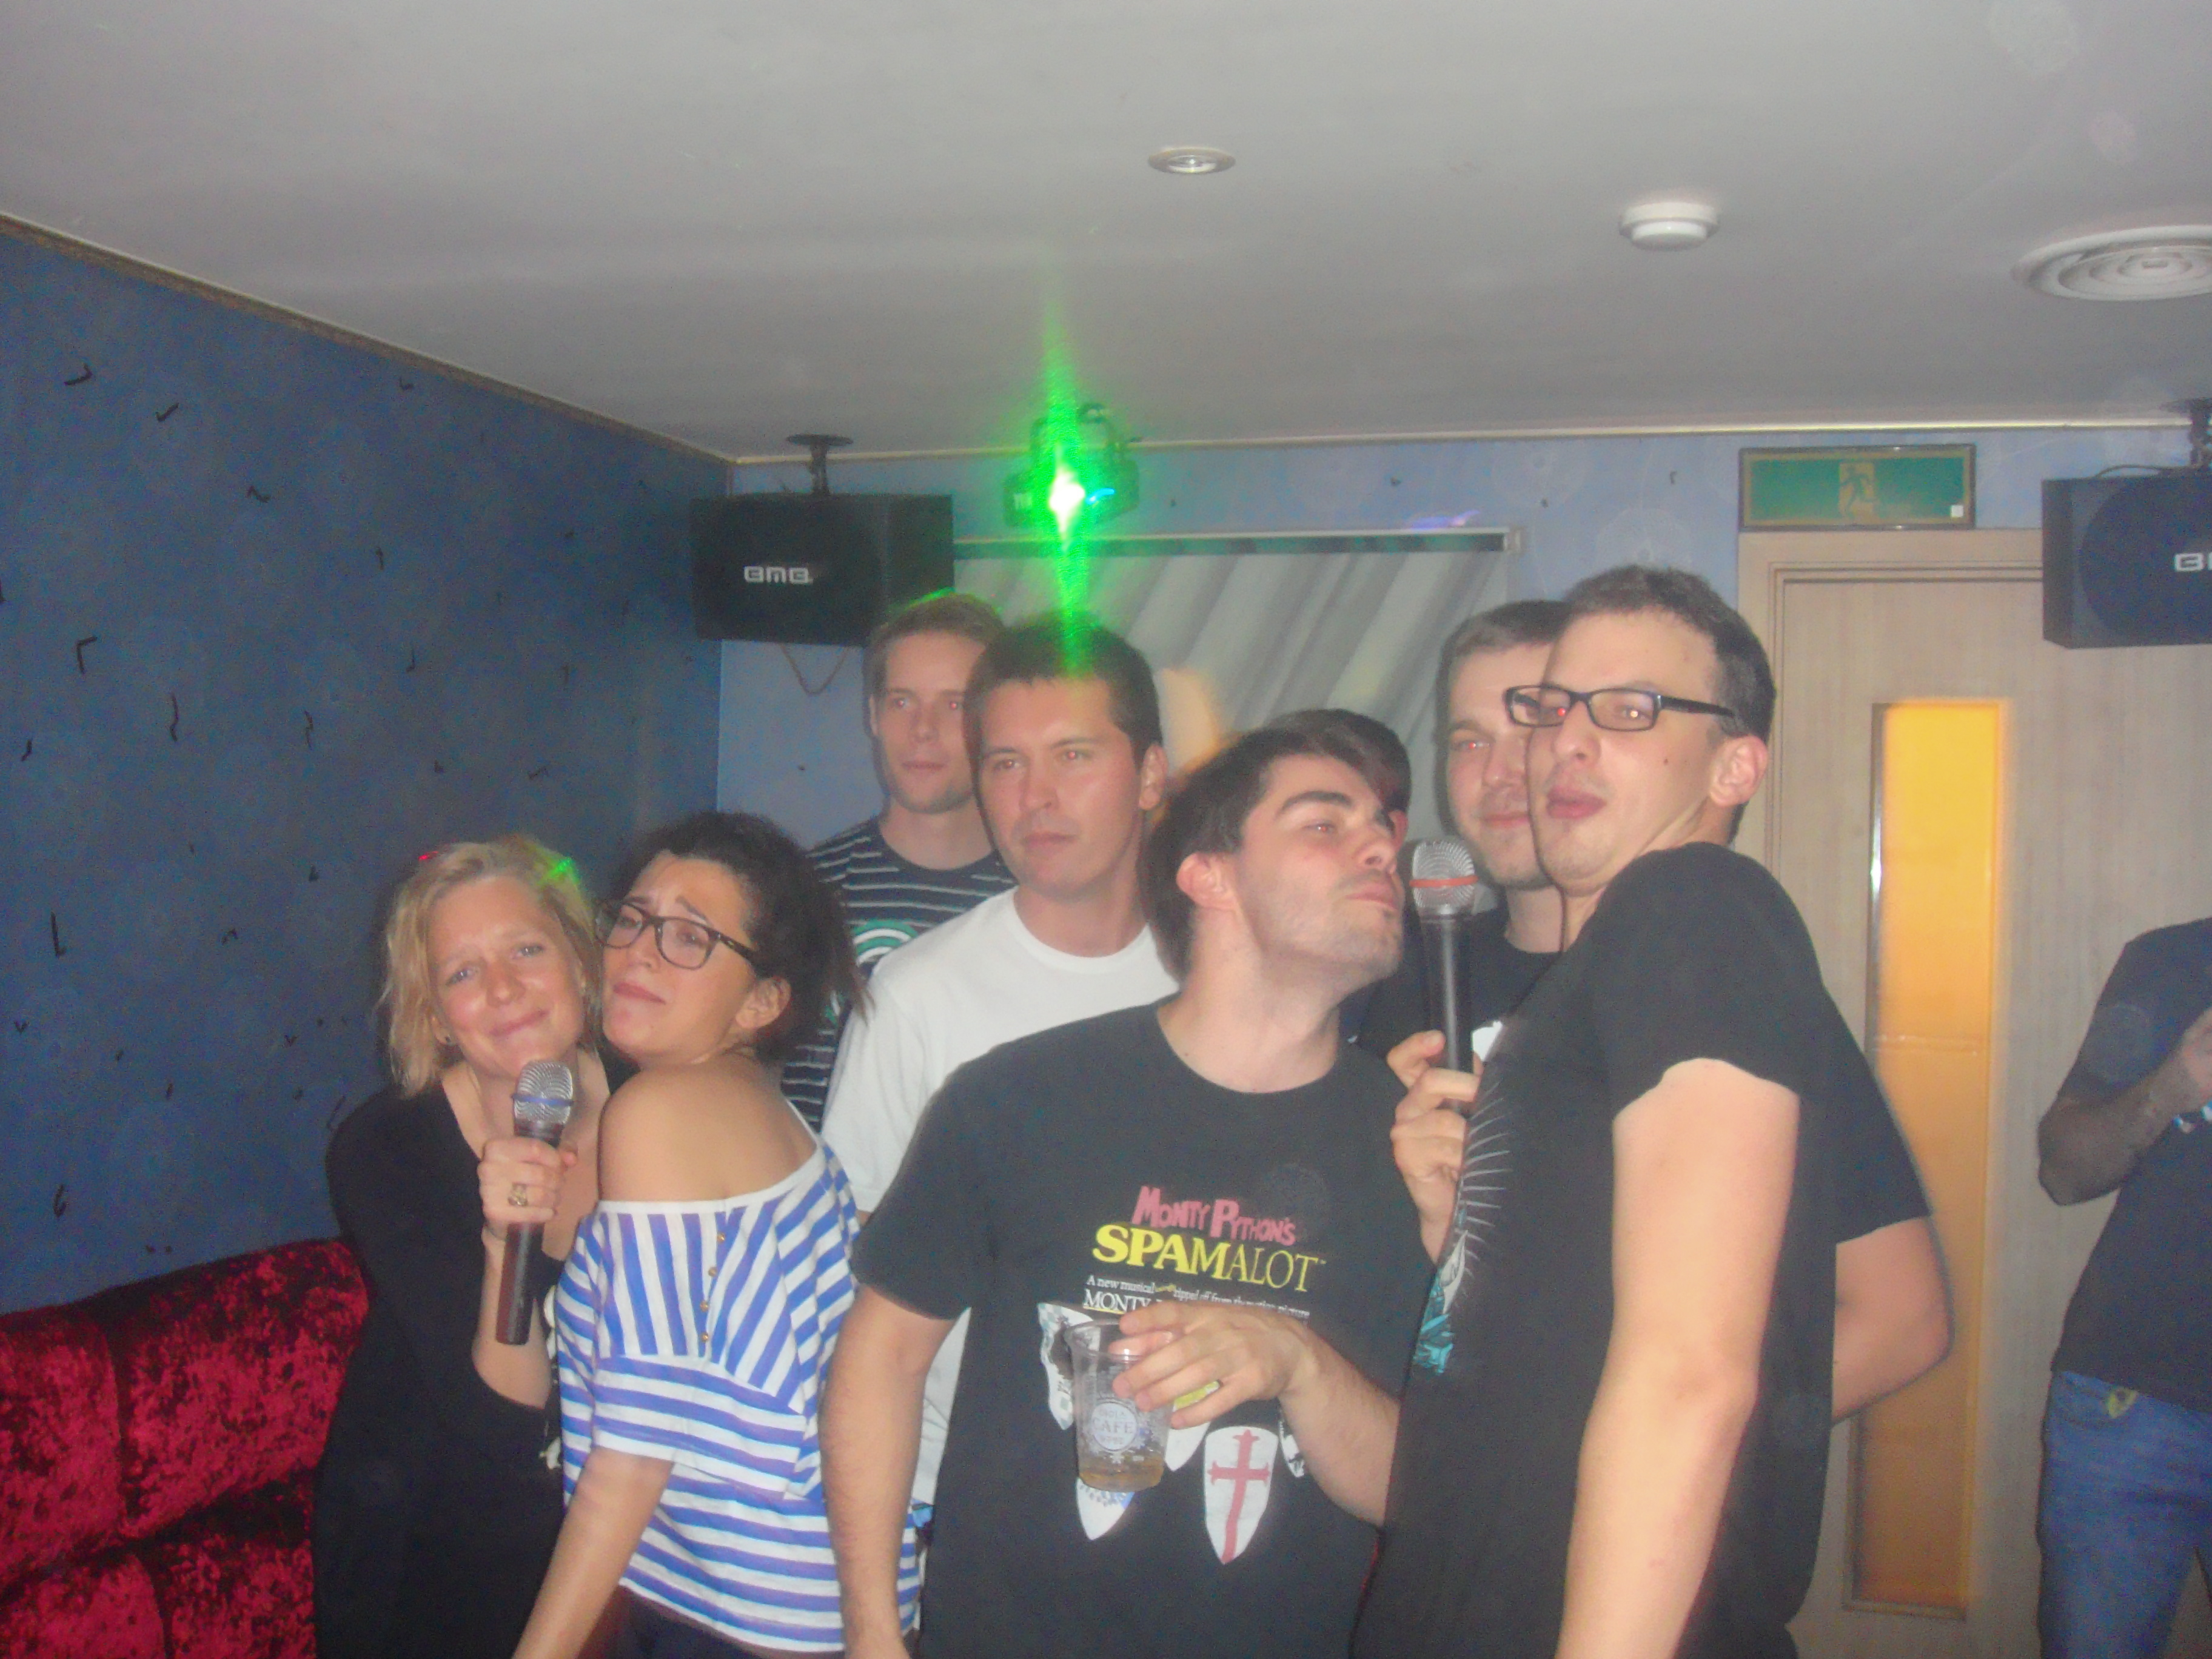
\includegraphics[width=0.43\textwidth]{photos/10/07/DSC02442.jpg}}}
\caption{KAIST Business School rockstars}
\end{figure}

We planned to spend around 2 hours there. We ended up singing for 4 hours straight, before our vocal cords gave up and turned us into a group of whispering rockstars. During the evening, we went through all the ``classics'' such as Queen, The Grease, ABBA, U2 or Backstreet Boys (\textit{``I Want It That Way''} by Mark and me was simply the best performance of the evening.), as well as some contemporary crap such as Justin Bieber (\textit{``Baby, Baby, Baby, Oooooooh!''}), Wiz Khalifa or Justin Timberlake. We also drank a ridiculous amount of beer and soju, but that's just what you do.

At 2am we finally finished, partly because we were tired and partly because there was no more beer in the place. Yes, we drank it all. Each of us paid 20,000KRW (\EUR{12}), which is fairly cheap for the amount of fun (and alcohol) we had, and went home or to the Burger King for a little snack. The next day I was barely able to speak, but it was definitely worth it, because:

\begin{blockquote}Am I your fire,\\
your one desire,\\
believe when I say,\\
I want it that way\end{blockquote}

	\end{content}
\end{post}
